%% bare_jrnl.tex
%% V1.4b
%% 2015/08/26
%% by Michael Shell
%% see http://www.michaelshell.org/
%% for current contact information.
%%
%% This is a skeleton file demonstrating the use of IEEEtran.cls
%% (requires IEEEtran.cls version 1.8b or later) with an IEEE
%% journal paper.
%%
%% Support sites:
%% http://www.michaelshell.org/tex/ieeetran/
%% http://www.ctan.org/pkg/ieeetran
%% and
%% http://www.ieee.org/

%%*************************************************************************
%% Legal Notice:
%% This code is offered as-is without any warranty either expressed or
%% implied; without even the implied warranty of MERCHANTABILITY or
%% FITNESS FOR A PARTICULAR PURPOSE! 
%% User assumes all risk.
%% In no event shall the IEEE or any contributor to this code be liable for
%% any damages or losses, including, but not limited to, incidental,
%% consequential, or any other damages, resulting from the use or misuse
%% of any information contained here.
%%
%% All comments are the opinions of their respective authors and are not
%% necessarily endorsed by the IEEE.
%%
%% This work is distributed under the LaTeX Project Public License (LPPL)
%% ( http://www.latex-project.org/ ) version 1.3, and may be freely used,
%% distributed and modified. A copy of the LPPL, version 1.3, is included
%% in the base LaTeX documentation of all distributions of LaTeX released
%% 2003/12/01 or later.
%% Retain all contribution notices and credits.
%% ** Modified files should be clearly indicated as such, including  **
%% ** renaming them and changing author support contact information. **
%%*************************************************************************


\documentclass[journal,onecolumn]{IEEEtran}

\usepackage{cite}
\usepackage{caption}
\usepackage{amsmath}
\usepackage{algorithm}
\usepackage[noend]{algpseudocode}
\usepackage{array}
\usepackage{graphicx}
\usepackage{float}

% correct bad hyphenation here
\hyphenation{op-tical net-works semi-conduc-tor}


\begin{document}
\title{Case Study: Implementing the Particle Swarm Optimization algorithm and comparison with other metaheuristics}

\author{Wilbert~Pumacay,~\textit{Catholic University San Pablo},~wilbert.pumacay@ucsp.edu.pe\\
        Gerson~Vizcarra,~\textit{Catholic University San Pablo},~gerson.vizcarra@ucsp.edu.pe}

% make the title area
\maketitle

% As a general rule, do not put math, special symbols or citations
% in the abstract or keywords.
\begin{abstract}
Heuristic-based swarm algorithms emerged as a powerful family of optimization techniques, inspired by the collective behavior of social animals. Particle Swarm Optimization (PSO) , part of this family, is known to solve large-scale nonlinear optimization problems using particles as a set of candidate solutions. In this paper we test the PSO on 3 common benchmarks functions, present a parallel implementation of the algorithm, and compare it with the results from other metaheuristics using the Wilcoxon rank sum test. 
\\
\\
\end{abstract}

\begin{IEEEkeywords}
Metaheuristics, Particle Swarm Optimization, Convergence Behavior, CUDA.
\end{IEEEkeywords}



\section{ \textbf{Introduction} }

\IEEEPARstart{T}{he} Particle Swarm Optimization algorithm is a population-based optimization method. It is based on the social behavior of birds and fish when moving as a group and it has been applied to many areas, such as artificial neural network training, function optimization, fuzzy control, and pattern classification because of its ease of implementation and fast convergence to acceptable solutions.

\section{ \textbf{Particle Swarm Optimization (PSO)} }
\subsection{ \textbf{Basic concepts} }
Particle Swarm Optimization, first introduced by Kennedy and Eberhart \cite{Kennedy1995} is a stochastic optimization technique that is based on two fundamental disciplines·\cite{delValle2008}: social science and computer science. In addition, PSO uses the swarm intelligence concept: the collective behavior of unsophisticated agents that are interacting locally with their environment to create coherent global functional patterns.

\subsection{ \textbf{Description of the algorithm} }
PSO is a population based optimization technique, where the population is called a \textit{swarm}. Earch particle represents a posible solution to the optimization task at hand. During each iteration each particle accelerates in the direction of its own personal best solution found so far, as well as the direction of the global best solution discovered so far by any of the particles in the swarm, as described in Fig. 1. This means that if a particle found a promising new solution, the other particles will move closer to it. The whole algorithm can be described in Algorithm 1.
\\
\begin{figure}[H]
\centering
\captionsetup{justification=centering}
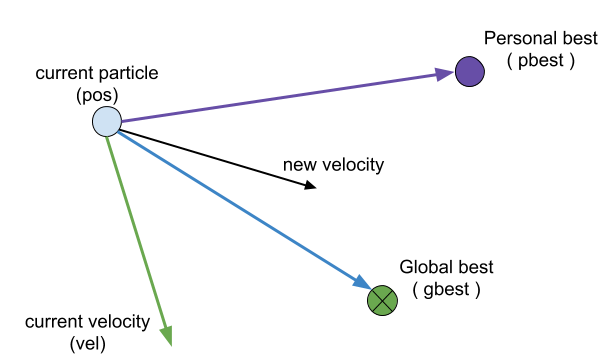
\includegraphics[width=3.0in]{_img/img_PSO_overview.png}
\caption{PSO overview}
\end{figure}

\begin{algorithm}
    \caption{Particle Swarm Optimization Algorithm}\label{alg:PSOpseudocode}
    \begin{algorithmic}[1]
        \State $\textbf{In}: \textit{objFunction, populationSize, w, $c_{1}$, $c_{2}$, k}$
        \State $\textbf{Out}: \textit{Solution optima } P_{g.cost}$
        \State $P_{g.pos} = \textbf{0}$
        \State $P_{g.cost} = Inf$
        \State $particles = \textbf{CreateParticles()}$
        \While {$\textit{ !stopCondition() }$}
            \For {$p$ {\bfseries in} $particles$}
                \State $\textbf{UpdateParticlesVelocities()}$
                \State $\textbf{UpdateParticlesPositions()}$
                \State $\textbf{UpdatePersonalBest()}$
                \State $\textbf{UpdateGlobalBest()}$
            \EndFor
        \EndWhile
        \\
        \Return $P_{g.cost}$
    \end{algorithmic}
\end{algorithm}

Each individual particle has the following attributes: 
\\
\begin{itemize}
    \item A current position in search space $x$.
    \item A current velocity $v$.
    \item A personal best position in the search space $x^{pbest}$.\\
\end{itemize}
As desribed earlier, each particle updates its velocity according to its personal best and the global best. The update rule (based in the social behaviour mentioned earlier ) can be described with the following equation:
\\
\begin{equation} \label{eq:1}
    \begin{aligned}
    v \leftarrow w v + c_{1} r_{1} [x^{pbest} - x] + c_{2} r_{2} [x^{gbest} - x]
    \end{aligned}
\end{equation}
\\
Where $w$ (inertia coefficient ), $c_{1}$ (cognitive coefficient ), $c_{2}$ (social coefficient ) and $k$ are the hyperparameters of the algorithm; and $r_{1}$ and $r_{2}$ are random numbers in the range $[0, 1]$. We then just update the particle position with the just calculated velocity.
\\
\begin{equation} \label{eq:2}
    \begin{aligned}
        x \leftarrow x + v.
    \end{aligned}
\end{equation}
\\
The personal best position of each particle, $x^{pbest}$ is updated using the following equation :
\\
\begin{equation} \label{eq:3}
  \begin{aligned}
    x^{pbest} \leftarrow x, &&\textit{if } Cost(x)\leq Cost(x^{pbest})
  \end{aligned}
\end{equation}
\\
and the global best solution found by any particle during all previous steps, $x^{gbest}$, is defined as :

\begin{equation} \label{eq:4}
    \begin{aligned}
        x^{gbest}=arg\min_{x}( Cost(x) )
    \end{aligned}
\end{equation}

\subsection{ \textbf{Implementation details} }

The algorithm is quite easy to implement, and that is one reason why it is still used. We implemented both a serial and a parallel version of the algorithm and test it using manually tuned hyperparameters. The best configuration that work in our case was :
\\
\begin{gather}
    w = 1.0,c_{1} = 2.0, c_{2} = 2.0, k = 0.5, populationSize = 100000
\end{gather}
\\
For the CPU implementation we followed a simple variation of the asynchronous PSO algorithm, which is described in Algorithm 2; and for the GPU implementation we followed the same variation of the PSO algorithm in a synchronous way, by making the comparison with the global best outside of the particles update loop. Both implementations are shown in figures 2 and 3.

\begin{figure}[H]
\centering
\captionsetup{justification=centering}
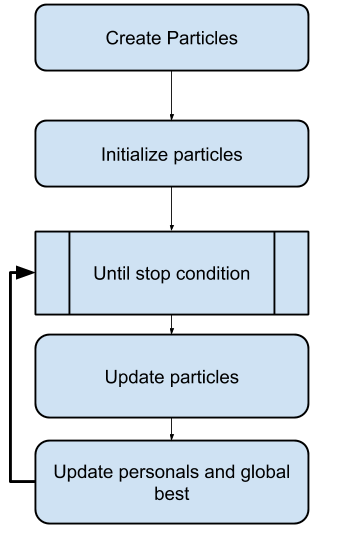
\includegraphics[width=2.5in,height=3.5in]{_img/img_PSO_algorithm_cpu.png}
\caption{PSO cpu implementation}
\end{figure}

\begin{figure}[H]
\centering
\captionsetup{justification=centering}
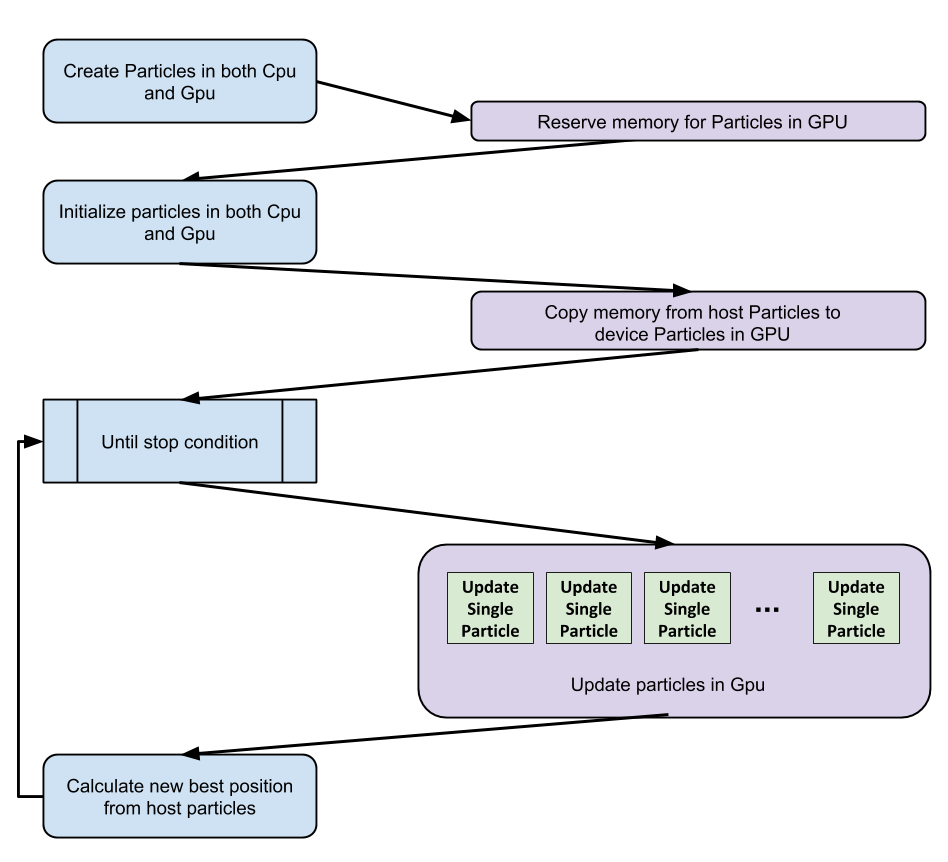
\includegraphics[width=4.5in,height=4.5in]{_img/img_PSO_algorithm_gpu.png}
\caption{PSO gpu implementation}
\end{figure}

\begin{algorithm}[H]
    \caption{Particle Swarm Optimization - Asynchonous Serial Version}\label{alg:PSOcpu}
    \begin{algorithmic}[1]
        \State $\textbf{In}: \textit{objFunction, populationSize, w, $c_{1}$, $c_{2}$, k, dimensions, domain}$
        \State $\textbf{Out}: \textit{Solution optima } P_{g.cost}$
        \State $vMin = -k * ( domain.max - domain.min ) / 2.0$
        \State $vMax =  k * ( domain.max - domain.min ) / 2.0$
        \State $P_{g.pos} = \textit{zeros( dimensions )}$ \Comment{Position that gives best cost}
        \State $P_{g.cost} = Inf$ \Comment{Best cost so far}
        \\
        \State $Particles=\lbrace \rbrace$ \Comment{Empty array of particles}
        \For {$i=1$ {\bfseries to} $PopulationSize$} \Comment{Particles Initialization}
            \State $p = \textbf{Particle()}$
            \State $p.pos = \textbf{randUniform( domain )}$
            \State $p.vel = \textbf{zeros( dimensions )}$
            \State $p.cost = \textbf{objFunction( p.pos )}$
            \State $p.bestpos = p.pos$
            \State $p.bestcost = p.cost$
            \If {$p.cost \leq P_{g.cost}$}
                \State $P_{g.cost} = p.cost$
                \State $P_{g.pos} = p.pos$
            \EndIf
        \EndFor
        \\
        \While {$\textit{ !stopCondition() }$} \Comment{Optimization process}
            \For {$p$ {\bfseries in} $Particles$}
                \State $p.vel = w * p.vel + 
                                c_{1} * ( p.bestpos - p.pos ) + 
                                c_{2} * ( P_{g.pos} - p.pos )$ \Comment{Velocity update}
                \State $p.vel = \textbf{ClampVector}\textit{( p.vel, vMin, vMax )}$
                \State $p.pos = p.pos + p.vel$ \Comment{Position update}
                \State $p.pos = \textbf{ClipPosition}\textit{( p.pos, domain )}$
                \\
                \If {$p.cost \leq p.bestcost$}
                    \State $p.bestcost = p.cost$ \Comment{Update personal best}
                    \State $p.bestpos = p.pos$
                    \If {$p.cost \leq P_{g.cost}$}
                        \State $P_{g.cost} = p.cost$ \Comment{Update global best}
                        \State $P_{g.pos} = p.pos$
                    \EndIf
                \EndIf
            \EndFor
        \EndWhile
        \\
        \Return $P_{g.cost}$
    \end{algorithmic}
\end{algorithm}

\begin{algorithm}[H]
    \caption{Particle Swarm Optimization - Synchonous Parallel Gpu Version}\label{alg:PSOgpu}
    \begin{algorithmic}[1]
        \State $\textbf{In}: \textit{objFunction, populationSize, w, $c_{1}$, $c_{2}$, k, dimensions, domain}$
        \State $\textbf{Out}: \textit{Solution optima } P_{g.cost}$
        \State $vMin = -k * ( domain.max - domain.min ) / 2.0$
        \State $vMax =  k * ( domain.max - domain.min ) / 2.0$
        \State $P_{g.pos} = \textit{zeros( dimensions )}$ \Comment{Position that gives best cost}
        \State $P_{g.cost} = Inf$ \Comment{Best cost so far}
        \\
        \State $hostParticles = \lbrace \rbrace$
        \State $deviceParticles = \lbrace \rbrace$
        \State $\textbf{GpuCreateParticles}\textit{( hostParticles, deviceParticles, objFunction, populationSize, dimensions, domain )}$
        \State $\textbf{GpuInitParticles}\textit{( hostParticles, deviceParticles, objFunction )}$
        \\
        \While {$\textit{ !stopCondition() }$} \Comment{Optimization process}
            \State $\textbf{GpuUpdateParticles}\textit{( hostParticles, deviceParticles, w, $c_{1}$, $c_{2}$, k )}$s
            \For {$p$ {\bfseries in} $hostParticles$}
                \If {$p.cost \leq P_{g.cost}$}
                    \State $P_{g.cost} = p.cost$ \Comment{Update global best}
                    \State $P_{g.pos} = p.pos$
                \EndIf
            \EndFor
        \EndWhile
        \Return $P_{g.cost}$
    \end{algorithmic}
\end{algorithm}

\begin{algorithm}[H]
    \caption{Particle Swarm Optimization - GpuUpdateParticles}\label{alg:PSOgpu_kernel_updateparticles}
    \begin{algorithmic}[1]
        \State $\textbf{In}: \textit{deviceParticles, coreIndx, w, $c_{1}$, $c_{2}$, k, $P_{g}$}$
        \State $p = \textbf{getDeviceParticle}\textit{( coreIndx )}$
        \State $p.vel = w * p.vel + 
                        c_{1} * ( p.bestpos - p.pos ) + 
                        c_{2} * ( P_{g.pos} - p.pos )$ \Comment{Velocity update}
        \State $p.vel = \textbf{ClampVector}\textit{( p.vel, vMin, vMax )}$
        \State $p.pos = p.pos + p.vel$ \Comment{Position update}
        \State $p.pos = \textbf{ClipPosition}\textit{( p.pos, domain )}$
        \\
        \If {$p.cost \leq p.bestcost$}
            \State $p.bestcost = p.cost$ \Comment{Update personal best}
            \State $p.bestpos = p.pos$
        \EndIf
    \end{algorithmic}
\end{algorithm}

\section{ \textbf{Results} }
To test our implementation, we used the following benchmark functions :
\\
\begin{enumerate}
    \item \textbf{Ackley}: This is a function with a minimum global optima at $\textbf{X} = (0,0,\hdots)$ with cost of $0.0$.

    \begin{figure}[H]
    \centering
    \captionsetup{justification=centering}
    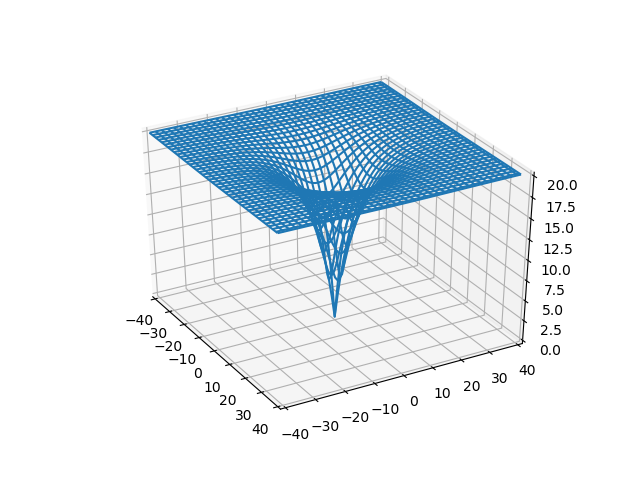
\includegraphics[width=3.6in]{_img/img_bmfunction_ackley.png}
    \caption{Ackley benchmark function}
    \end{figure}

    \item \textbf{Schwefel}: This is a function with a minimum global optima at $\textbf{X} = (420.9687,420.9687    ,\hdots)$ with cost of $0.0$.

    \begin{figure}[H]
    \centering
    \captionsetup{justification=centering}
    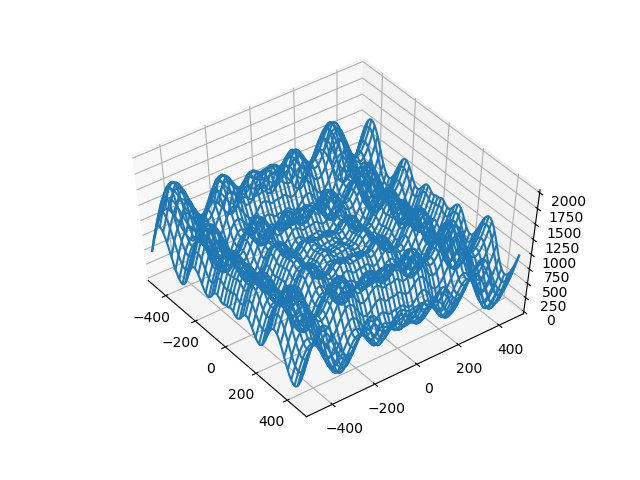
\includegraphics[width=3.6in]{_img/img_bmfunction_schwefel.jpeg}
    \caption{Schwefel benchmark function}
    \end{figure}

    \item \textbf{Schaffer6}: This is a function with a maximum optima at $\textbf{X} = (0,0,\hdots)$ with cost of $1.0$.

    \begin{figure}[H]
    \centering
    \captionsetup{justification=centering}
    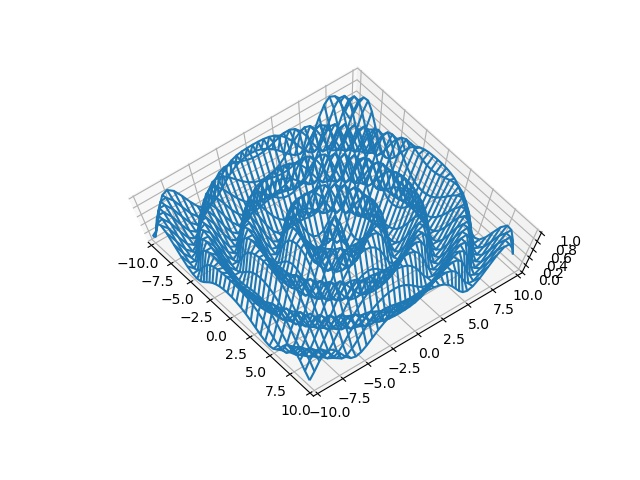
\includegraphics[width=3.6in]{_img/img_bmfunction_schafferfcn6.jpeg}
    \caption{Schaffer6 benchmark function}
    \end{figure}

\end{enumerate}

\subsection{ \textbf{Convergence behaviour} }

We tested the implementation for both 2 and 8 dimensions of the search space. In the case of 2 dimensions, we plotted the results in the surface and contour curves, and got the following behaviour:
\begin{figure}[H]
\centering
\captionsetup{justification=centering}
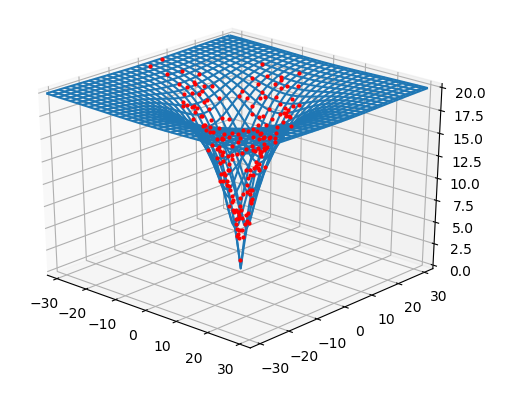
\includegraphics[width=3.0in]{_img/img_PSO_test_2d_ackley_3dview.png}
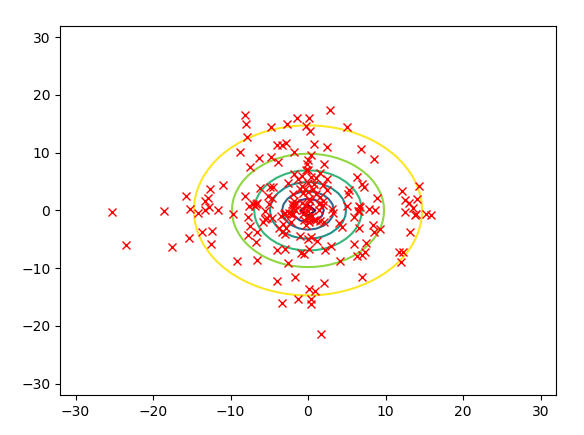
\includegraphics[width=3.0in]{_img/img_PSO_test_2d_ackley_contours.png}
\caption{Particles behaviour for the Ackley benchmark functions}
\end{figure}

\begin{figure}[H]
\centering
\captionsetup{justification=centering}
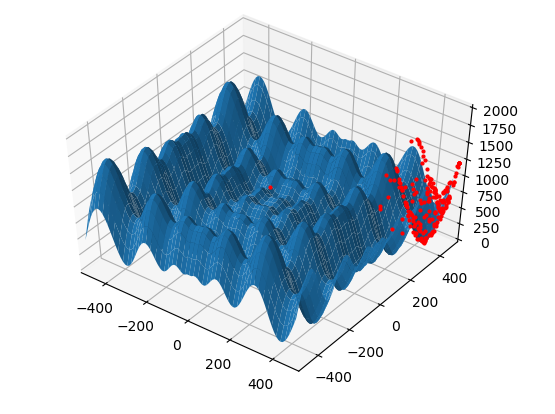
\includegraphics[width=3.0in]{_img/img_PSO_test_2d_schwefel_3dview.png}
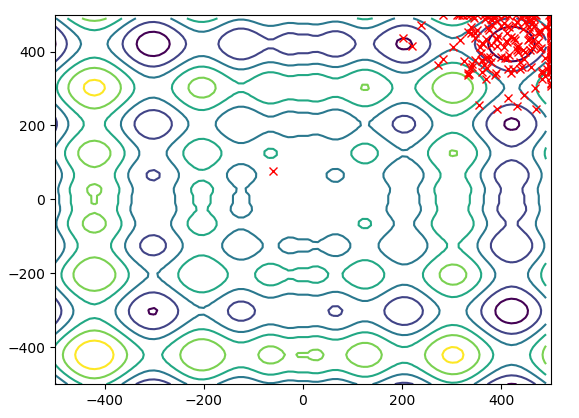
\includegraphics[width=3.0in]{_img/img_PSO_test_2d_schwefel_contours.png}
\caption{Particles behaviour for the Schwefel benchmark functions}
\end{figure}

\begin{figure}[H]
\centering
\captionsetup{justification=centering}
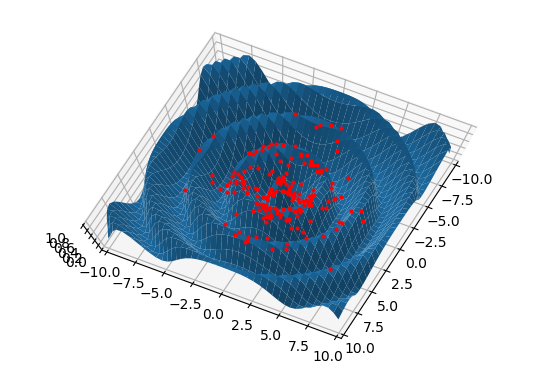
\includegraphics[width=3.0in]{_img/img_PSO_test_2d_schafferfcn6_3dview.png}
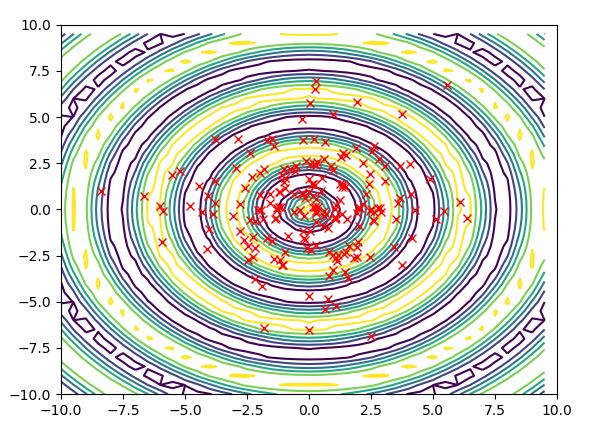
\includegraphics[width=3.0in]{_img/img_PSO_test_2d_schafferfcn6_contours.png}
\caption{Particles behaviour for the Schaffer6 benchmark functions}
\end{figure}

Also, we plotted the optima at each iteration for both 2d and 8d, and got the following results :

\begin{figure}[H]
\centering
\captionsetup{justification=centering}
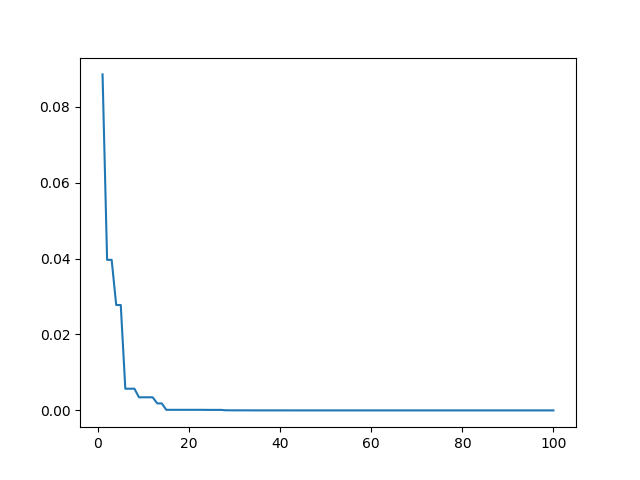
\includegraphics[width=3.0in]{_img/img_PSO_convergence_ackley_2d.png}
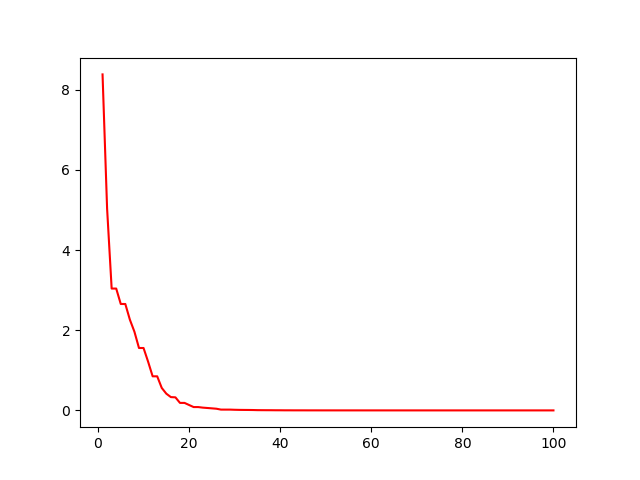
\includegraphics[width=3.0in]{_img/img_PSO_convergence_ackley_8d.png}
\caption{Convergence behaviour during optimization in the Ackley function. Left: 2d, Right: 8d}
\end{figure}

\begin{figure}[H]
\centering
\captionsetup{justification=centering}
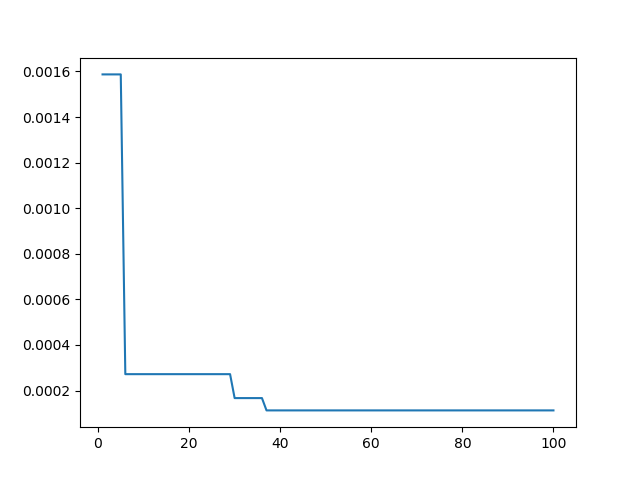
\includegraphics[width=3.0in]{_img/img_PSO_convergence_schwefel_2d.png}
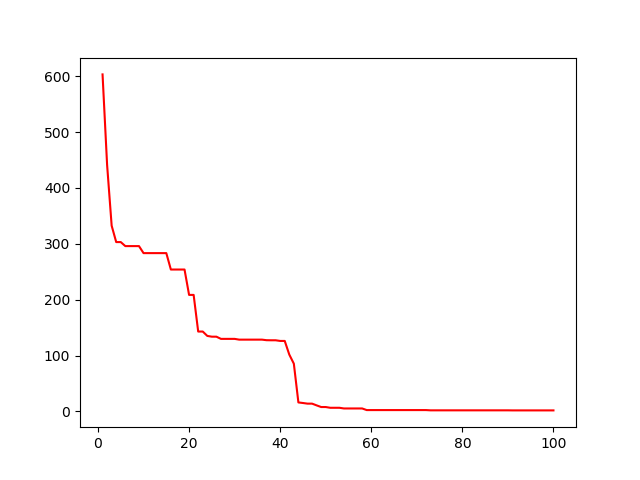
\includegraphics[width=3.0in]{_img/img_PSO_convergence_schwefel_8d.png}
\caption{Convergence behaviour during optimization in the Schwefel function. Left: 2d, Right: 8d}
\end{figure}

\begin{figure}[H]
\centering
\captionsetup{justification=centering}
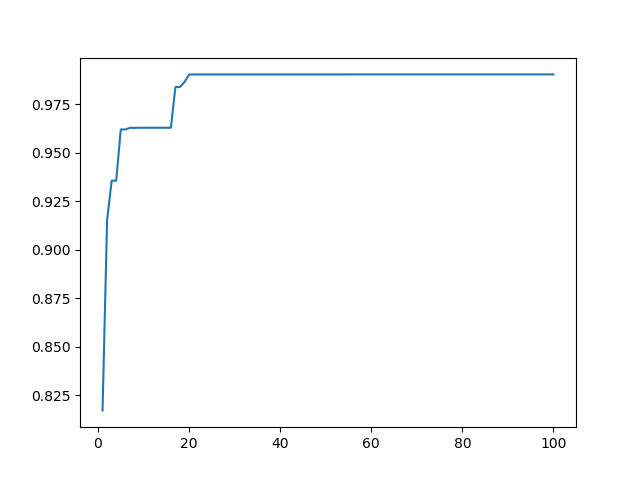
\includegraphics[width=3.0in]{_img/img_PSO_convergence_schaffer6_2d.png}
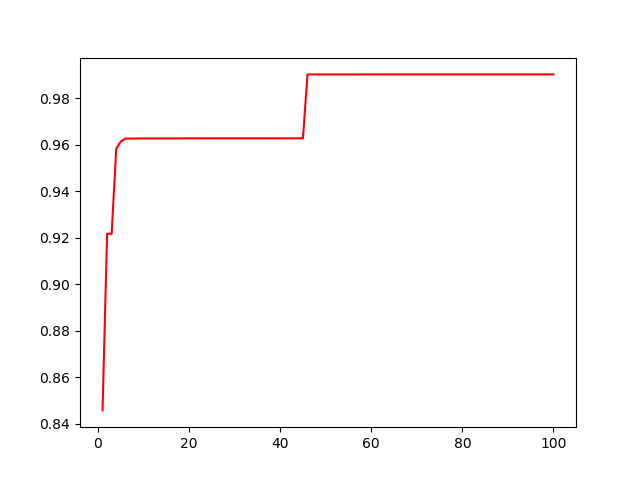
\includegraphics[width=3.0in]{_img/img_PSO_convergence_schaffer6_8d.png}
\caption{Convergence behaviour during optimization in the Schaffer function. Left: 2d, Right: 8d}
\end{figure}

\subsection{ \textbf{Comparison with other metaheuristics} }

We run the Wilcoxon test to compare our implementation with the following metaheuristics :

\begin{itemize}

    \item \textbf{CS} Cuckoo Search algorithm
    \item \textbf{BA} Bat Inspired algorithm
    \item \textbf{GC} GENOCOP algorithm
    \item \textbf{FPA} Flower Pollination algorithm
    \item \textbf{DE} Dynamic Differential Evolution algorithm
    \item \textbf{GSA} Gravitational Search algorithm
    \item \textbf{HS} Harmony Search algorithm
    \item \textbf{GWO} Grey Wolf Optimization algorithm

\end{itemize}

The \textbf{p-val} found by running the Wilcoxon test in \textbf{Octave} (with a vector of 100 executions) can be found in the following table.

\textbf{~}\\
\begin{tabular}{|c|c|c|c|c|c|c|}

\hline \textbf{Algoritmo} & \textbf{Ackely 2d} & \textbf{Ackely 8d} & \textbf{Schewfel 2d} & \textbf{Schewfel 8d} & \textbf{Schaffer6 2d} & \textbf{Schaffer6 8d} \\\hline

CS      & 3.89656e-18   & 3.89656e-18   & 0             & 0           & 3.45096e-16  & 0.00393593 \\\hline
BA      & 0             & 3.89656e-18   & 4.01616e-18   & 0.0114986   & 1.78129e-17  & 7.69167e-10\\\hline
GC      & 3.89656e-18   & 3.89656e-18   & 0             & 0           & 0            & 3.89656e-18\\\hline
FPA     & 3.89656e-18   & 3.89656e-18   & 0             & 0           & 3.45096e-16  & 3.89656e-18\\\hline
DE      & 3.89656e-18   & 2.61518e-12   & 0             & 0           & 1.1236e-11   & 3.89656e-18\\\hline
GSA     & 3.89656e-18   & 3.89656e-18   & 2.28706e-14   & 9.86809e-16 & 0            & 0          \\\hline
HS      & 3.89656e-18   & 3.89656e-18   & 3.36398e-13   & 2.14496e-10 & 0            & 0          \\\hline
GWO     & 3.89656e-18   & 3.89656e-18   & 7.5806e-06    & 3.89656e-18 & 0            & 0\\\hline

\end{tabular}

\section{Conclusions}

\begin{itemize}

    \item The algorithm works quite fast in finding an optima. As the results suggest, the algorithm finds a local optima quite fast, but it gets stuck in that optima, as the other particles are attracted to that optima. Once that optima is found, the exploration is restricted to the neighborhood of that optima, which does not allow to escape it in cases of complicated objective functions.

    \item One way to escape the optima is by using more particles, which was an option in our CUDA implementation. This allows us to search the space in order to escape local optima, as was the case of the Schwefel function, in which we got stuck because of lack of a bigger population size in our first test when tuning the hyperparameters.

\end{itemize}

\begin{thebibliography}{1}

\bibitem{Kennedy1995}
  James Kennedy and Russell Eberhart. \\
  \textit{Particle Swarm Optimization.} - 1995
\\
\bibitem{Garnier2007}
  Simon Garnier, Jacques Gautrais, Guy Theraulaz\\
  \textit{The biological principles of swarm intelligence.} - 2007
\\
\bibitem{delValle2008}
  Yamille del Valle, Ganesh Kumar, Salman Mohagheghi, Jean Hernandez, Ronald Harley\\
  \textit{Particle Swarm Optimization: Basic Concepts, Variants and Applications in Power Systems.} - 2008

\end{thebibliography}

\end{document}


